% Running Header
{\noindent\hfill\textsf{\textbf{MỤC 2.4}}\quad\textsf{Định nghĩa chính xác của giới hạn}\hspace{1.5cm}\textbf{\textsf{107}}\par}
\vspace{10pt}

% Đoạn 1
\noindent
\begin{minipage}[t]{\margincolwidth}
  \vspace{0pt}
\end{minipage}%
\hspace{\colgutter}%
\begin{minipage}[t]{\maincolwidth}
  \vspace{0pt}
  \hspace*{14pt}Ta giải thích mệnh đề này theo quan điểm hình học bằng cách biểu diễn một hàm số bằng sơ đồ mũi tên như trong Hình~2, trong đó $f$ ánh xạ một tập con của $\mathbb{R}$ lên một tập con khác của $\mathbb{R}$.
\end{minipage}
\vspace{8pt}

% Hình 2
\noindent
\begin{minipage}[c]{\margincolwidth}
  \raggedleft
  \textbf{\textsf{HÌNH 2}}
\end{minipage}%
\hspace{\colgutter}%
\begin{minipage}[c]{\maincolwidth}
  \centering
  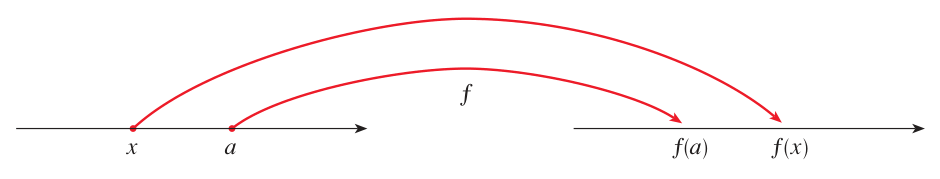
\includegraphics[width=0.88\linewidth]{images/p0142_fig1.png}
\end{minipage}
\vspace{8pt}

% Đoạn 2
\noindent
\begin{minipage}[t]{\margincolwidth}
  \vspace{0pt}
\end{minipage}%
\hspace{\colgutter}%
\begin{minipage}[t]{\maincolwidth}
  \vspace{0pt}
  \hspace*{14pt}Định nghĩa của giới hạn phát biểu rằng nếu cho trước bất kỳ khoảng nhỏ $(L - \varepsilon, L + \varepsilon)$ nào quanh $L$, thì ta có thể tìm được một khoảng $(a - \delta, a + \delta)$ quanh $a$ sao cho $f$ ánh xạ tất cả các điểm trong khoảng $(a - \delta, a + \delta)$ (ngoại trừ có thể là $a$) vào trong khoảng $(L - \varepsilon, L + \varepsilon)$. (Xem Hình~3.)
\end{minipage}
\vspace{8pt}

% Hình 3
\noindent
\begin{minipage}[c]{\margincolwidth}
  \raggedleft
  \textbf{\textsf{HÌNH 3}}
\end{minipage}%
\hspace{\colgutter}%
\begin{minipage}[c]{\maincolwidth}
  \centering
  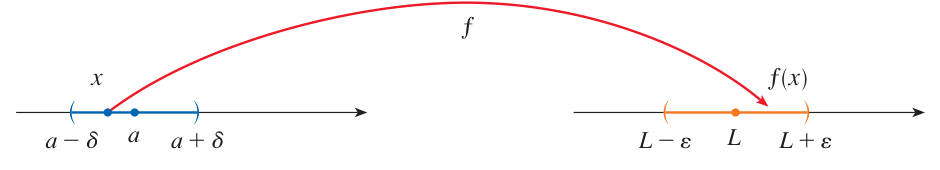
\includegraphics[width=0.88\linewidth]{images/p0142_fig2.png}
\end{minipage}
\vspace{8pt}

% Đoạn 3 & 4
\noindent
\begin{minipage}[t]{\margincolwidth}
  \vspace{0pt}
\end{minipage}%
\hspace{\colgutter}%
\begin{minipage}[t]{\maincolwidth}
  \vspace{0pt}
  \hspace*{14pt}Một cách giải thích hình học khác về giới hạn có thể được đưa ra dựa trên đồ thị của hàm số. Nếu cho trước $\varepsilon > 0$, ta vẽ các đường nằm ngang $y = L + \varepsilon$ và $y = L - \varepsilon$ cùng với đồ thị của $f$. (Xem Hình~4.) Nếu $\lim_{x \to a} f(x) = L$, thì ta có thể tìm được một số $\delta > 0$ sao cho nếu ta giới hạn $x$ nằm trong khoảng $(a - \delta, a + \delta)$ và lấy $x \neq a$, thì đường cong $y = f(x)$ sẽ nằm giữa hai đường thẳng $y = L - \varepsilon$ và $y = L + \varepsilon$. (Xem Hình~5.) Bạn có thể thấy rằng nếu một giá trị $\delta$ như vậy đã được tìm ra, thì bất kỳ giá trị $\delta$ nào nhỏ hơn cũng sẽ thỏa mãn.

  \vspace{6pt}
  \hspace*{14pt}Điều quan trọng cần nhận ra là quá trình được minh họa trong Hình~4 và Hình~5 phải đúng với \textit{mọi} số dương $\varepsilon$, bất kể nó được chọn nhỏ đến mức nào. Hình~6 cho thấy rằng nếu chọn một giá trị $\varepsilon$ nhỏ hơn, thì có thể cần một giá trị $\delta$ nhỏ hơn tương ứng.
\end{minipage}
\vspace{12pt}

% Cụm Hình 4, Hình 5, Hình 6 trải rộng toàn trang
\noindent
\begin{minipage}[t]{0.31\textwidth}
  \centering
  \vspace{0pt}
  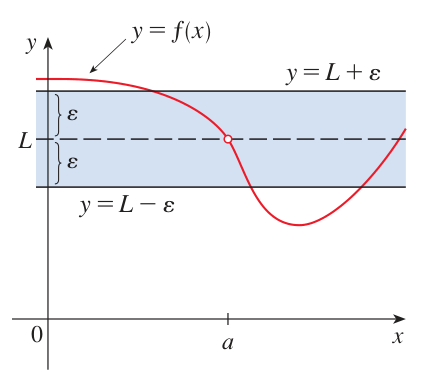
\includegraphics[width=\linewidth]{images/p0142_fig3.png}
\end{minipage}\hfill
\begin{minipage}[t]{0.34\textwidth}
  \centering
  \vspace{0pt}
  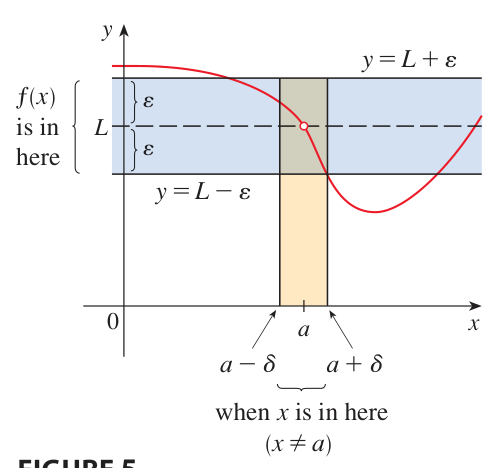
\includegraphics[width=\linewidth]{images/p0142_fig4.png}
\end{minipage}\hfill
\begin{minipage}[t]{0.31\textwidth}
  \centering
  \vspace{0pt}
  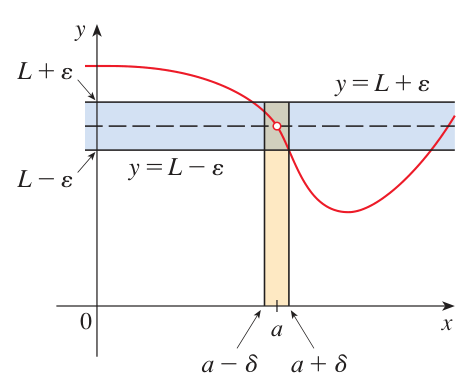
\includegraphics[width=\linewidth]{images/p0142_fig5.png}
\end{minipage}

\vspace{3pt}
\noindent
\begin{minipage}[t]{0.31\textwidth}
  \centering
  \textbf{\textsf{HÌNH 4}}
\end{minipage}\hfill
\begin{minipage}[t]{0.34\textwidth}
  \centering
  \textbf{\textsf{HÌNH 5}}
\end{minipage}\hfill
\begin{minipage}[t]{0.31\textwidth}
  \centering
  \textbf{\textsf{HÌNH 6}}
\end{minipage}
\vspace{12pt}

% Ví dụ 1
\noindent
\begin{minipage}[t]{\margincolwidth}
  \vspace{0pt}
\end{minipage}%
\hspace{\colgutter}%
\begin{minipage}[t]{\maincolwidth}
  \vspace{0pt}\noindent
  {\bfseries\color{stewartblue}\textsf{VÍ DỤ 1}}\quad Vì $f(x) = x^3 - 5x + 6$ là một đa thức, theo Tính chất Thế trực tiếp, ta biết rằng $\lim_{x \to 1} f(x) = f(1) = 1^3 - 5(1) + 6 = 2$. Hãy sử dụng đồ thị để tìm một số $\delta$ sao cho nếu khoảng cách từ $x$ đến $1$ nhỏ hơn $\delta$, thì khoảng cách từ $y$ đến $2$ nhỏ hơn $0{,}2$, tức là,
  \[
  \text{nếu}\qquad |x - 1| < \delta \qquad\text{thì}\qquad |(x^3 - 5x + 6) - 2| < 0{,}2
  \]
\end{minipage}

\vfill
% Footer bản quyền
{\centering\tiny\color{footercolor}
Copyright 2021 Cengage Learning. All Rights Reserved. May not be copied, scanned, or duplicated, in whole or in part. Due to electronic rights, some third party content may be suppressed from the eBook and/or eChapter(s).\\
Editorial review has deemed that any suppressed content does not materially affect the overall learning experience. Cengage Learning reserves the right to remove additional content at any time if subsequent rights restrictions require it.\par}
